\begin{figure}
	\centering
	\subfigure[$\Delta t$ = 1 día]{
	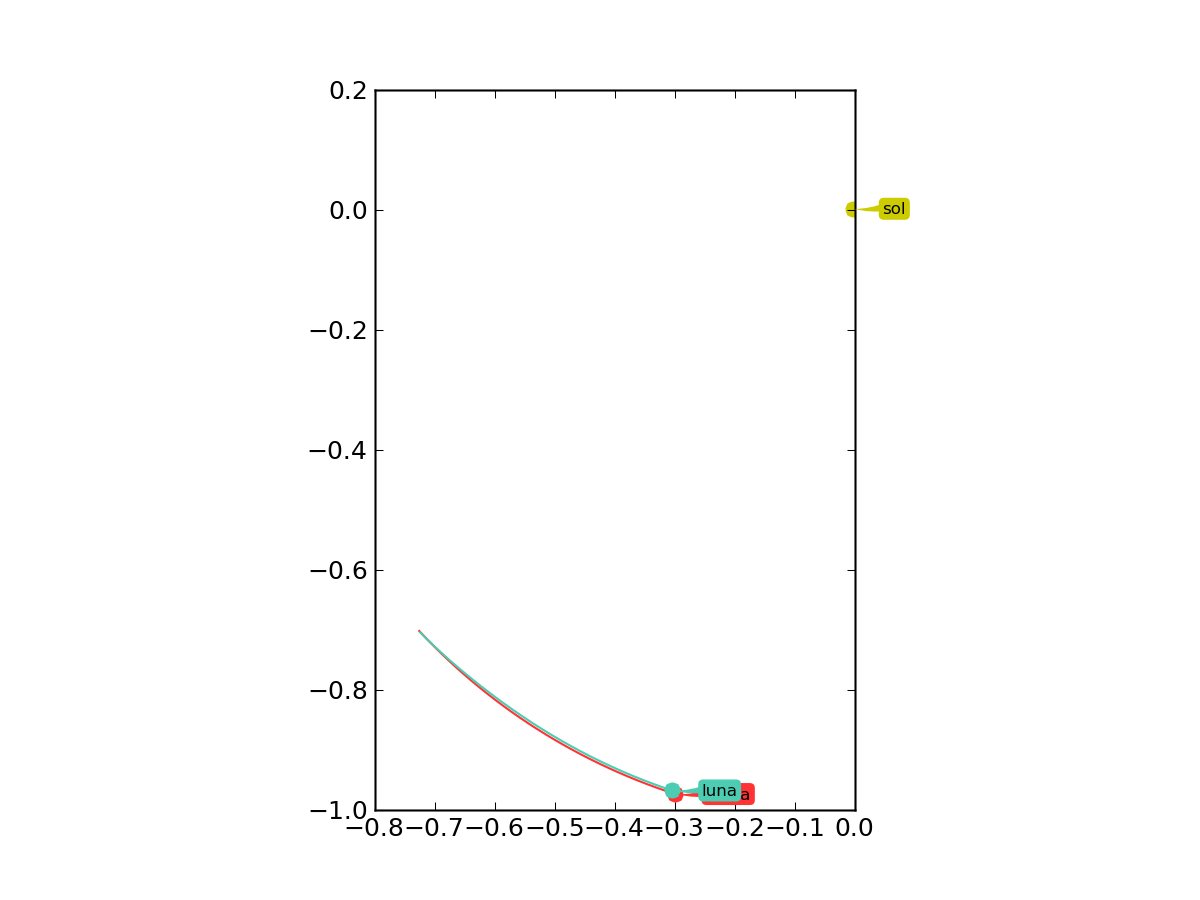
\includegraphics[scale=0.38]{img/ej1/metodo1/validacion_30_1.png}
	\label{fig:ej1_m1_30_1}
	}
	\subfigure[$\Delta t$ = 6 horas]{
	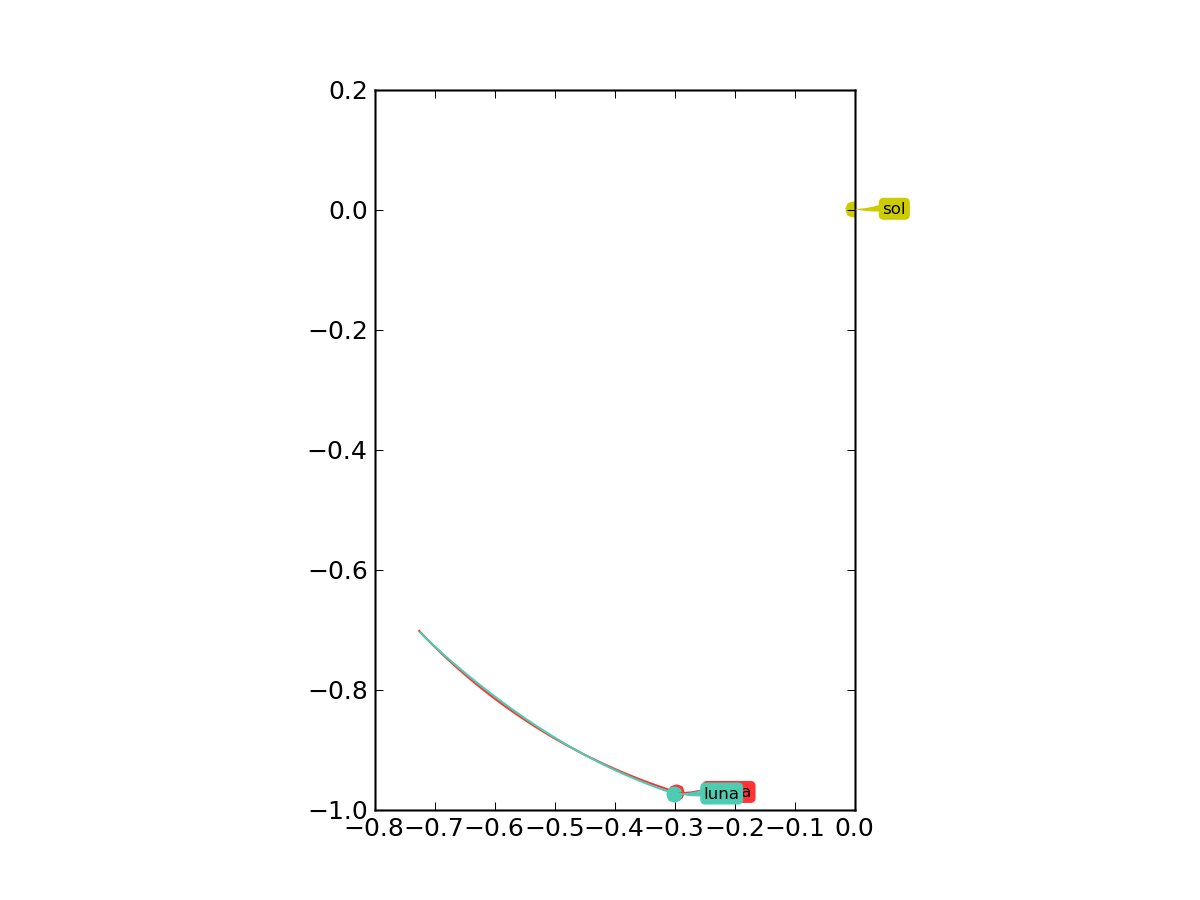
\includegraphics[scale=0.38]{img/ej1/metodo1/validacion_30_4.png}
	\label{fig:ej1_m1_30_4}
	}
	\\
	\subfigure[$\Delta t$ = 2 horas]{
	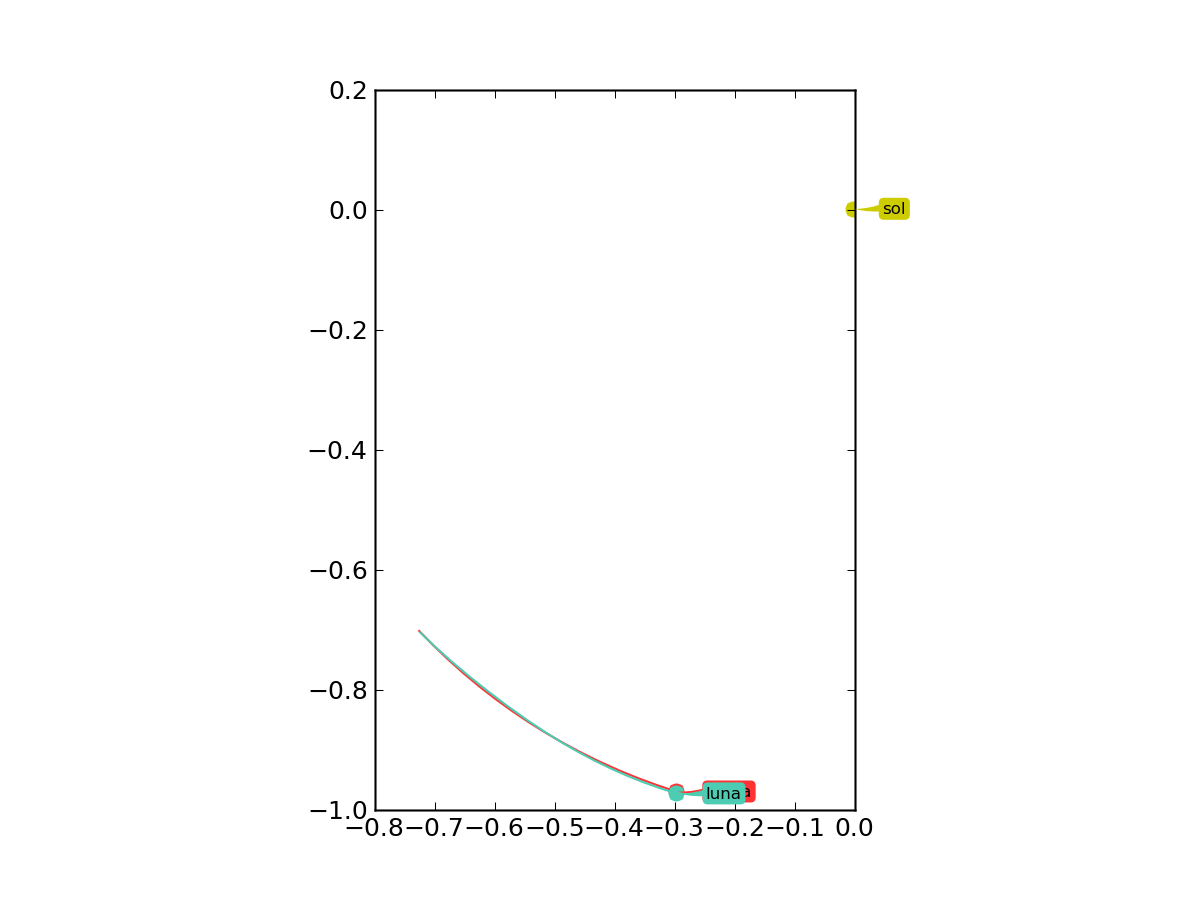
\includegraphics[scale=0.38]{img/ej1/metodo1/validacion_30_12.png}
	\label{fig:ej1_m1_30_12}
	}
	\subfigure[$\Delta t$ = 1 hora]{
	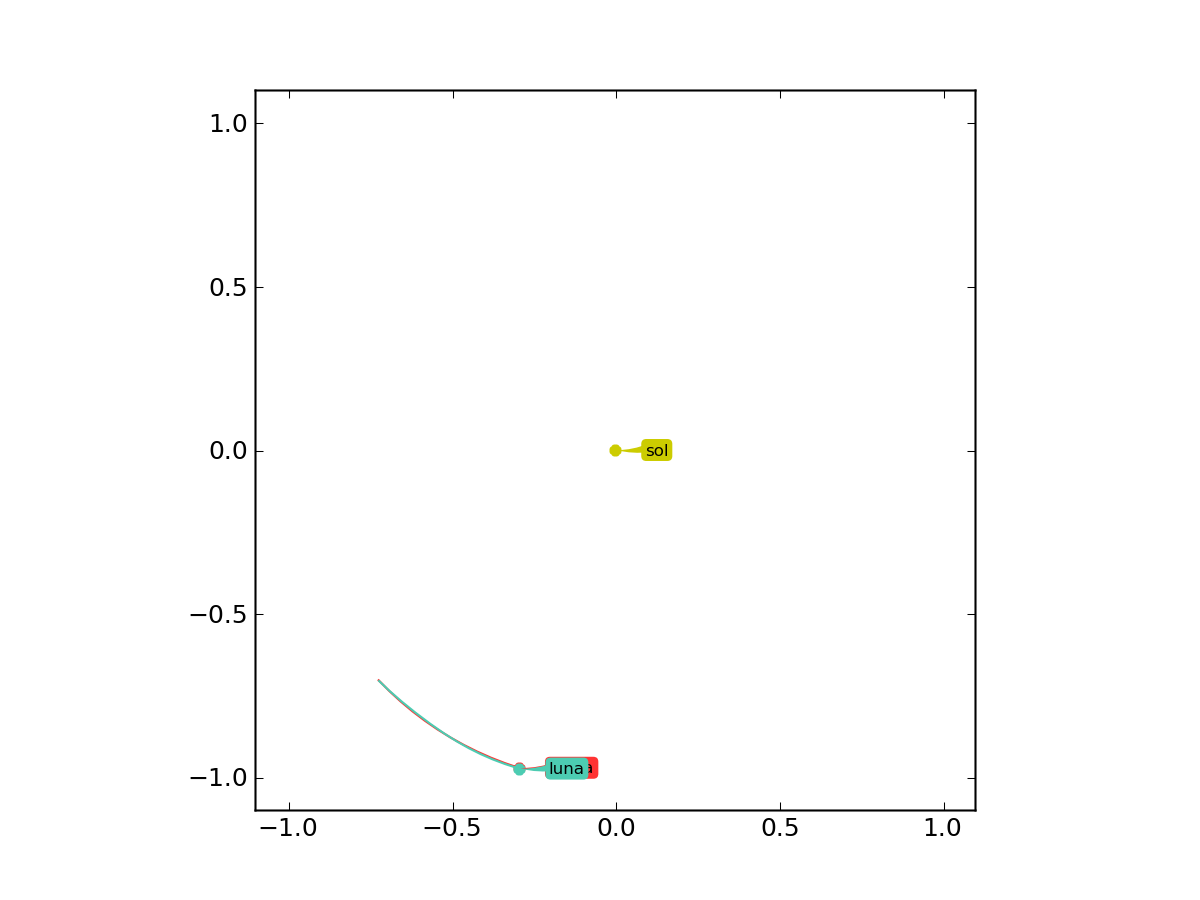
\includegraphics[scale=0.38]{img/ej1/metodo1/validacion_30_24.png}
	\label{fig:ej1_m1_30_24}
	}
	\caption{
		Simulación de validación del sistema sol$-$tierra$-$luna para un período de 30 días y distintos $\Delta t$
		con el método 1.
		Observamos que el error no parece ser tan grande a simple vista para este período.
	}
	\label{ fig:res_ej1_m1_30 }
\end{figure}
\begin{figure}
	\centering
	\subfigure[$\Delta t$ = 1 día]{
	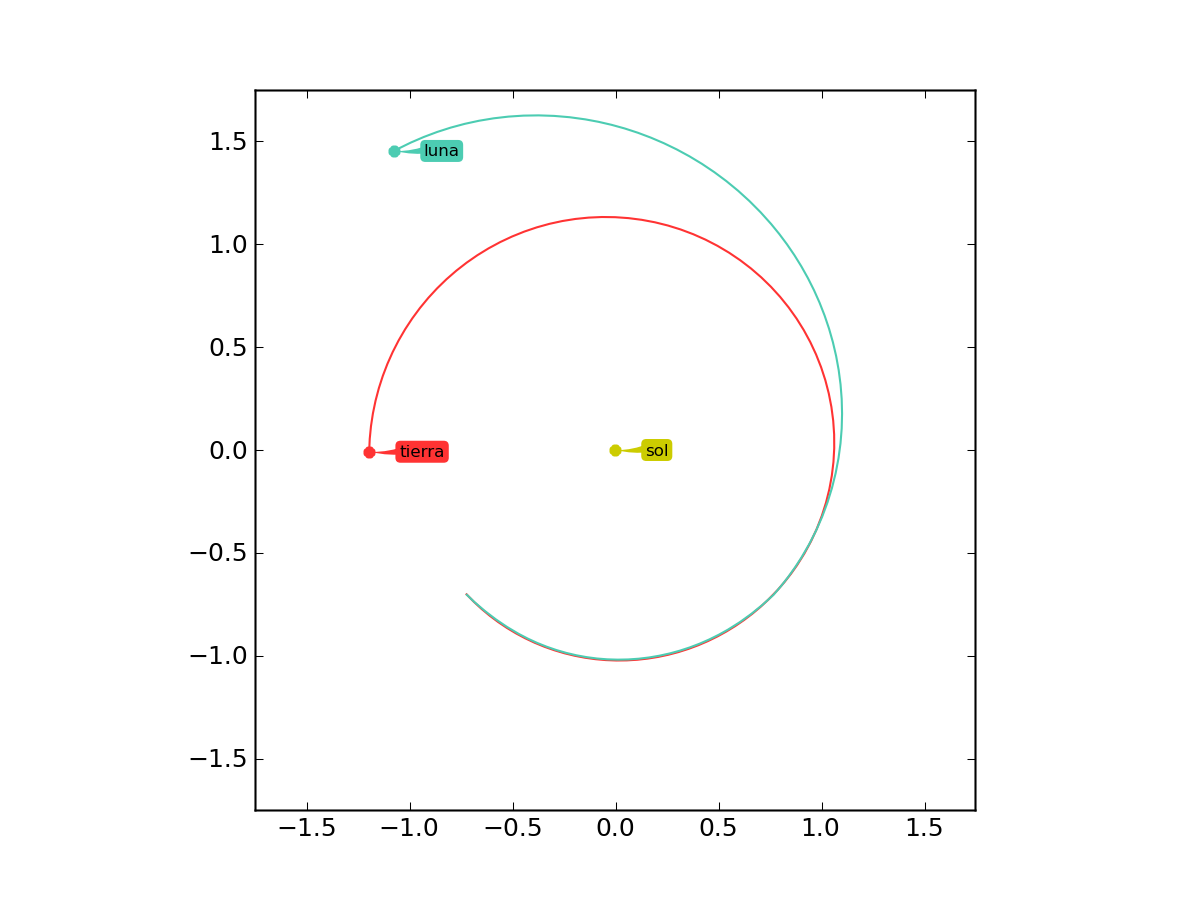
\includegraphics[scale=0.38]{img/ej1/metodo1/validacion_365_1.png}
	\label{fig:ej1_m1_365_1}
	}
	\subfigure[$\Delta t$ = 6 horas]{
	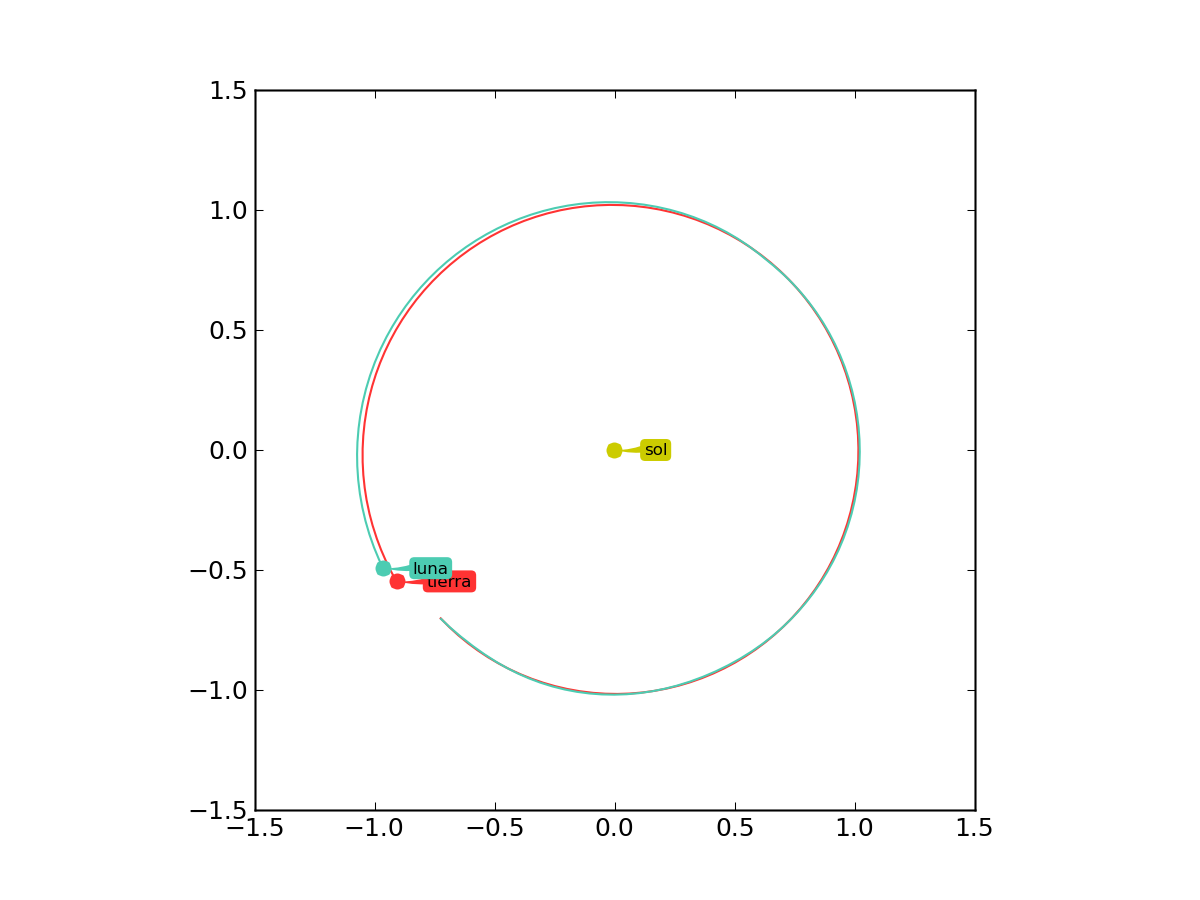
\includegraphics[scale=0.38]{img/ej1/metodo1/validacion_365_4.png}
	\label{fig:ej1_m1_365_4}
	}
	\\
	\subfigure[$\Delta t$ = 2 horas]{
	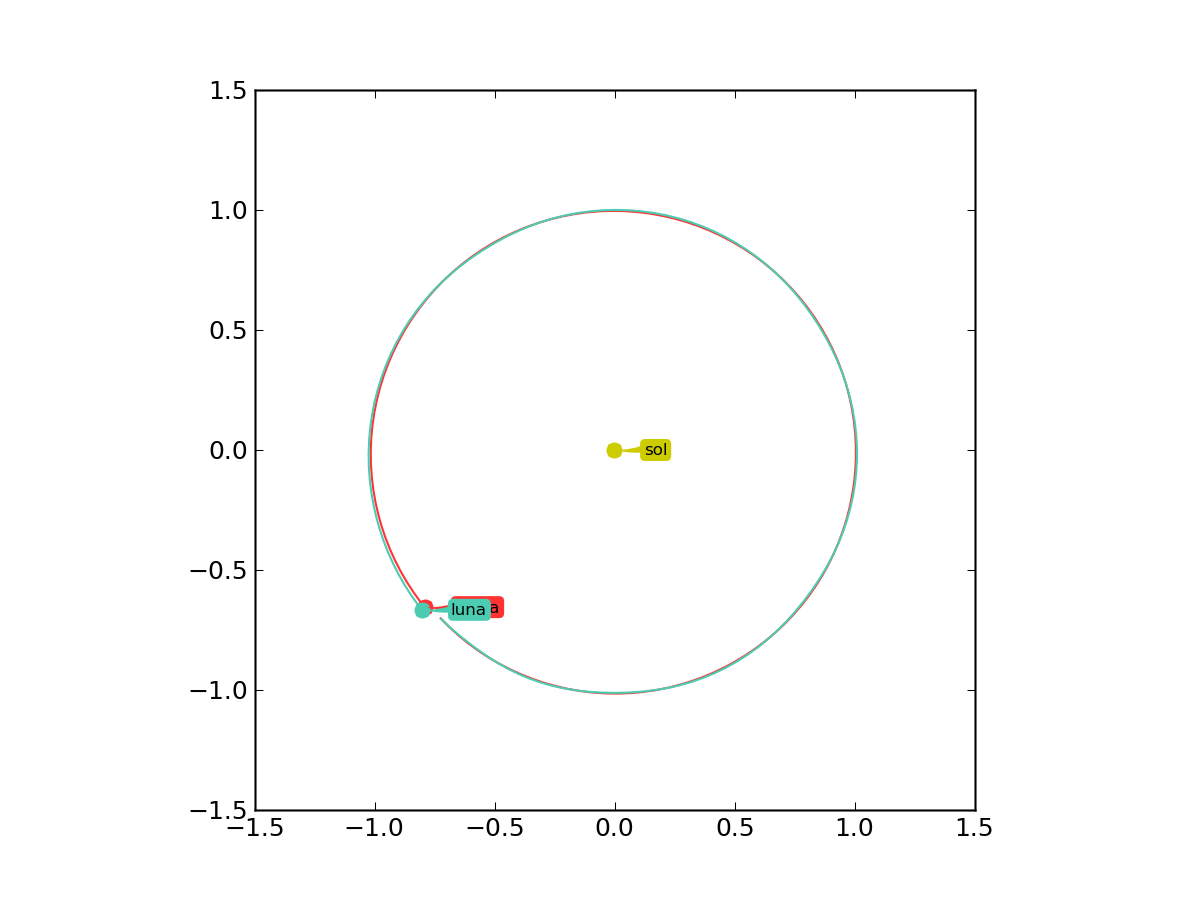
\includegraphics[scale=0.38]{img/ej1/metodo1/validacion_365_12.png}
	\label{fig:ej1_m1_365_12}
	}
	\subfigure[$\Delta t$ = 1 hora]{
	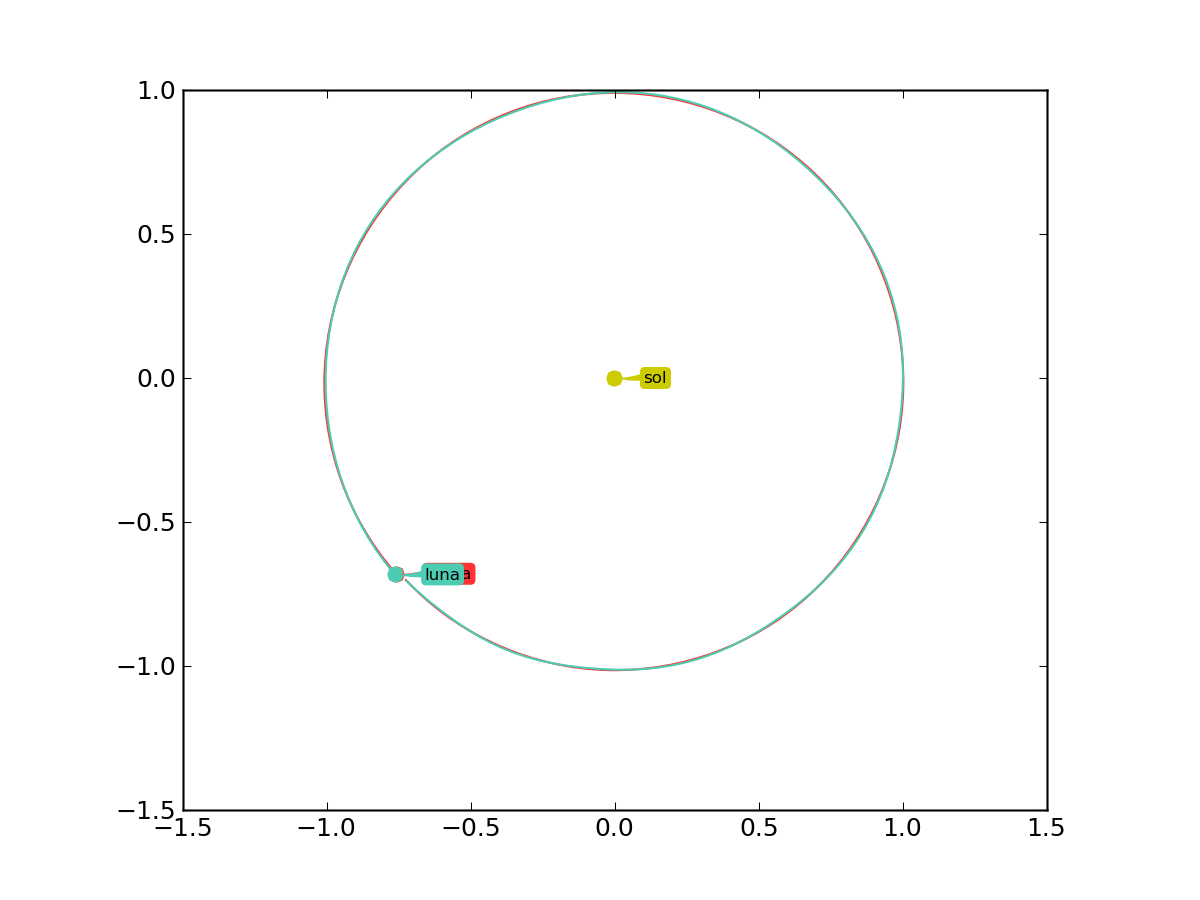
\includegraphics[scale=0.38]{img/ej1/metodo1/validacion_365_24.png}
	\label{fig:ej1_m1_365_24}
	}
	\caption{
		Simulación de validación del sistema sol$-$tierra$-$luna para un período de 1 año y distintos $\Delta t$
		con el método 1.
		Para esta cantidad de tiempo, la simulación con un $\Delta t$ de un día ya merece ser descartada.
		Las otras todavía parecen comportarse razonablemente
	}
	\label{ fig:res_ej1_m1_365 }
\end{figure}
\begin{figure}
	\centering
	\subfigure[$\Delta t$ = 1 día]{
	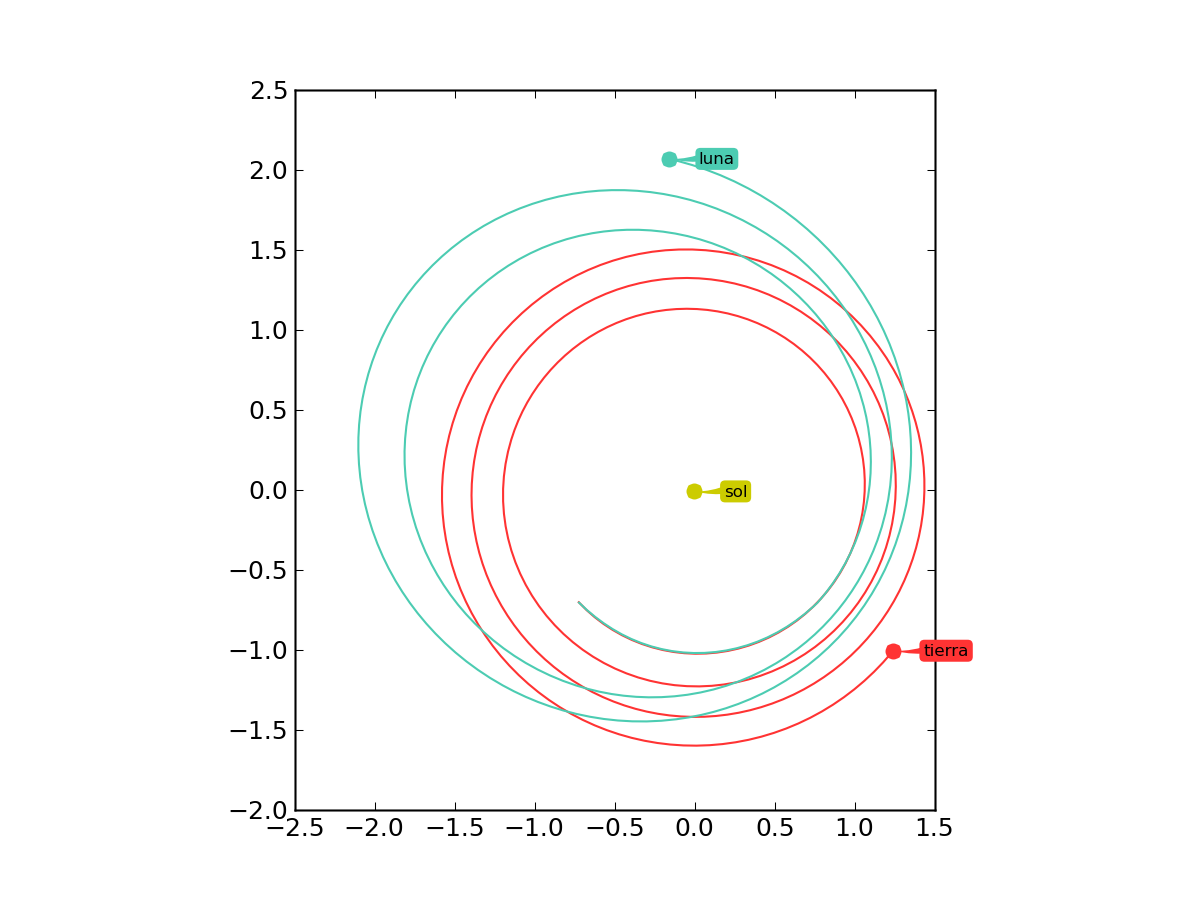
\includegraphics[scale=0.38]{img/ej1/metodo1/validacion_1825_1.png}
	\label{fig:ej1_m1_1825_1}
	}
	\subfigure[$\Delta t$ = 6 horas]{
	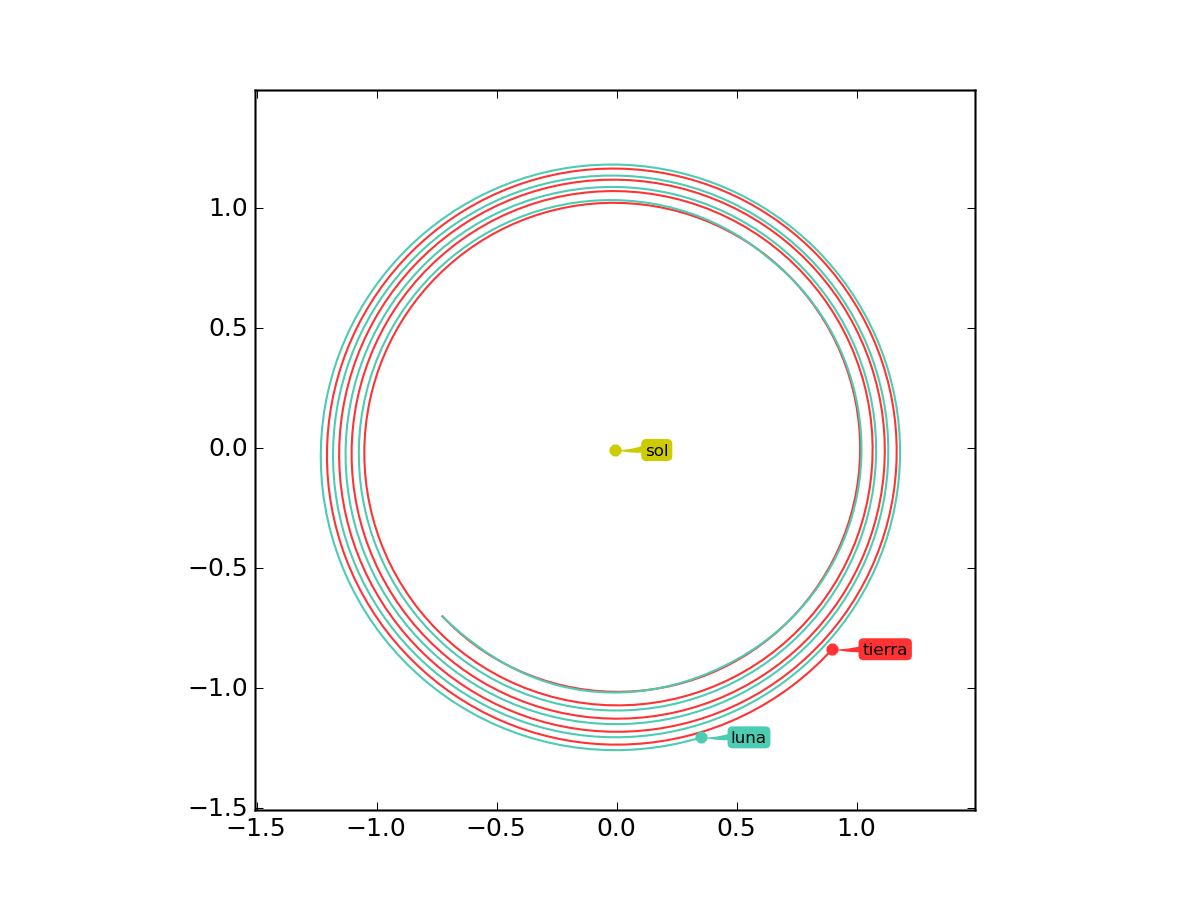
\includegraphics[scale=0.38]{img/ej1/metodo1/validacion_1825_4.png}
	\label{fig:ej1_m1_1825_4}
	}
	\\
	\subfigure[$\Delta t$ = 2 horas]{
	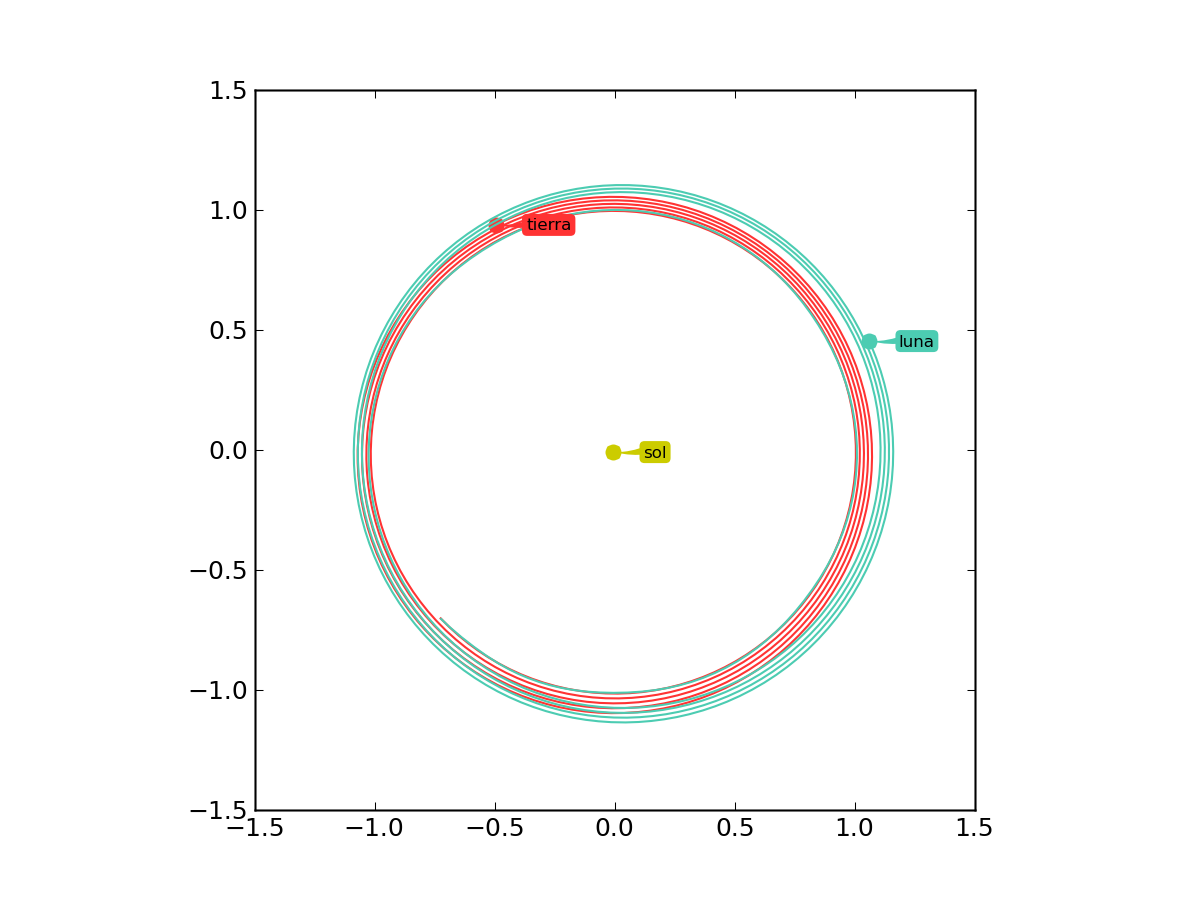
\includegraphics[scale=0.38]{img/ej1/metodo1/validacion_1825_12.png}
	\label{fig:ej1_m1_1825_12}
	}
	\subfigure[$\Delta t$ = 1 hora]{
	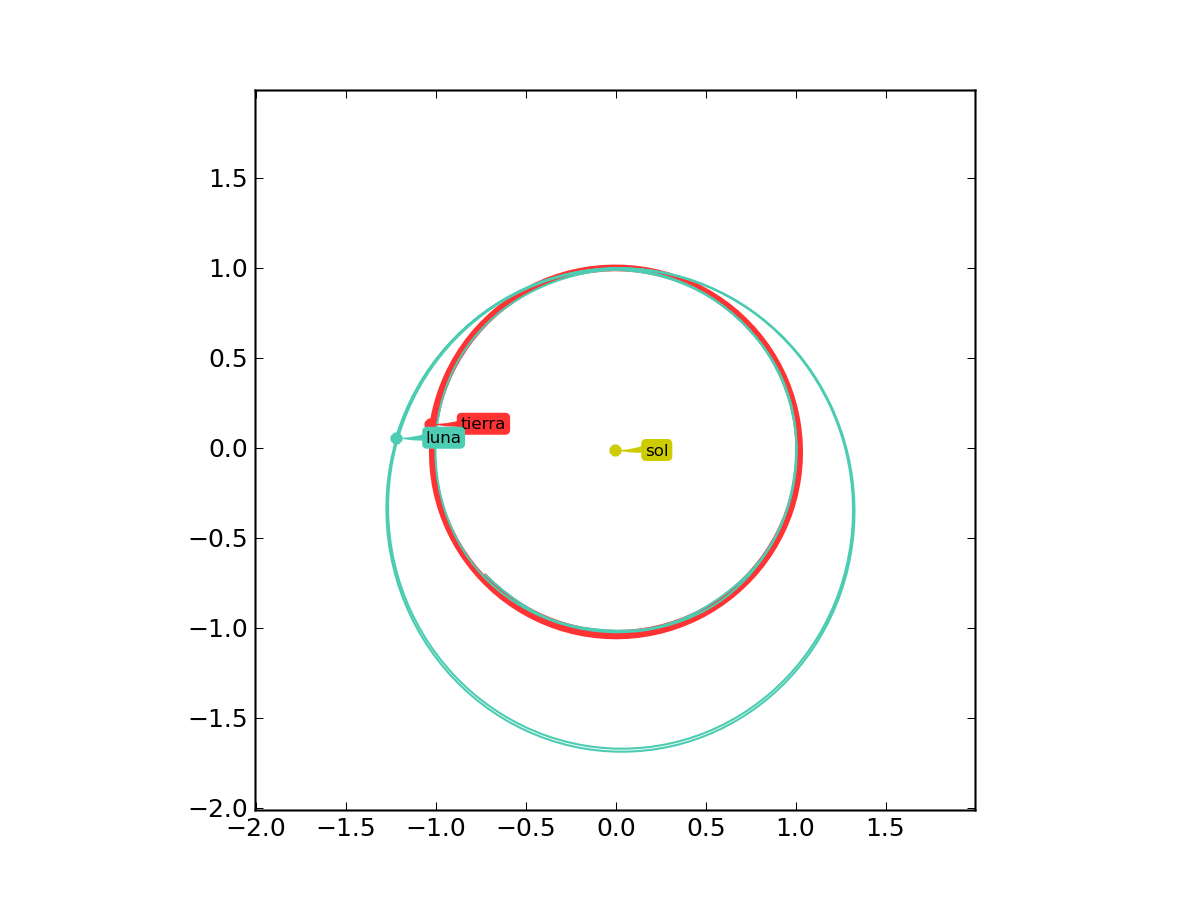
\includegraphics[scale=0.38]{img/ej1/metodo1/validacion_1825_24.png}
	\label{fig:ej1_m1_1825_24}
	}
	\caption{
		Simulación de validación del sistema sol$-$tierra$-$luna para un período de 5 años y distintos $\Delta t$
		con el método 1.
		Para esta cantidad de tiempo de simulación, las órbitas de los planetas ya comienzan a mostrar un movimiento espiral en vez de elíptico más de una vuelta.
		El mejor método parece ser el de $\Delta t$ de 2 horas, ya que para el de 1 hora la luna comienza a comportarse de una manera un poco mas extraña,
		comportamiento que atribuímos a errores de redondeo por tratar con numeros muy chicos o muy grandes al multiplicar o dividir respectivamente por un $\Delta t$ muy chico.
	}
	\label{ fig:res_ej1_m1_1825 }
\end{figure}
